\documentclass[aspectratio=169, 11pt]{beamer}

% ── Theme ───────────────────────────────────────────────────────
\usetheme{metropolis}
\usepackage{appendixnumberbeamer}
\usepackage{booktabs}
\usepackage{graphicx}
\usepackage{tikz}
\usetikzlibrary{
  positioning, arrows.meta, shapes.geometric,
  fit, backgrounds, calc
}
\usepackage{xcolor}
\usepackage{fontawesome5}

% ── Colours ─────────────────────────────────────────────────────
\definecolor{accent}{HTML}{0077B6}
\definecolor{airflowBg}{HTML}{017CEE}
\definecolor{pipelineBg}{HTML}{2E86C1}
\definecolor{minioBg}{HTML}{C72C48}
\definecolor{mlflowBg}{HTML}{0194E2}
\definecolor{apiBg}{HTML}{009688}
\definecolor{uiBg}{HTML}{FF4B4B}
\definecolor{k8sBg}{HTML}{326CE5}
\definecolor{infraBorder}{HTML}{B0BEC5}
\definecolor{storageBg}{HTML}{FFF3E0}
\definecolor{servingBg}{HTML}{E8F5E9}
\definecolor{orchBg}{HTML}{E3F2FD}
\definecolor{screenshotBg}{HTML}{F5F5F5}

\setbeamercolor{frametitle}{bg=accent, fg=white}
\setbeamercolor{progress bar}{fg=accent}

% ── Meta ────────────────────────────────────────────────────────
\title{Projet MLOps}
\subtitle{Pipeline de Classification 20 Newsgroups de Bout en Bout}
\author{}
\date{\today}
\institute{}

\begin{document}

% ================================================================
%  SLIDE 1 — Title
% ================================================================
\maketitle

% ================================================================
%  SLIDE 2 — Problem & Approach
% ================================================================
\begin{frame}{Probl\`eme \& Approche}
\small
\begin{columns}[T]
\begin{column}{0.5\textwidth}
\textbf{Objectif}\\[3pt]
Construire un syst\`eme ML \alert{pr\^et pour la production} qui~:
\begin{itemize}\setlength{\itemsep}{1pt}
  \item Classe du texte dans \textbf{20 cat\'egories}
  \item Se r\'eentra\^ine chaque semaine automatiquement
  \item Trace chaque exp\'erience pour la reproductibilit\'e
  \item Sert les pr\'edictions via une interface web
\end{itemize}

\vspace{0.3em}
\textbf{Jeu de donn\'ees} — 20 Newsgroups\\[2pt]
{\footnotesize ${\sim}18\,000$ entra\^inement / ${\sim}7\,500$ test\\
20 classes~: politique, sport, science, tech\dots}
\end{column}

\begin{column}{0.46\textwidth}
\textbf{\'Etapes du pipeline}\\[3pt]
{\small
\begin{enumerate}\setlength{\itemsep}{1pt}
  \item \textbf{T\'el\'echargement} — via scikit-learn
  \item \textbf{Pr\'etraitement} — nettoyage du texte
  \item \textbf{Entra\^inement} — 6 mod\`eles TF-IDF
  \item \textbf{Promotion} — champion si meilleur
\end{enumerate}
}

\vspace{0.3em}
\textbf{Mod\`eles entra\^in\'es par ex\'ecution}\\[2pt]
{\footnotesize
\begin{tabular}{@{}ll@{}}
\toprule
\textbf{Mod\`ele} & \textbf{Variantes} \\
\midrule
SGDClassifier & $\alpha{=}10^{-4},\; 10^{-3}$ \\
MultinomialNB & $\alpha{=}0.1,\; 1.0$ \\
LogisticRegression & $C{=}1,\; 10$ \\
\bottomrule
\end{tabular}
}
\end{column}
\end{columns}
\end{frame}

% ================================================================
%  SLIDE 3 — Architecture Diagram
% ================================================================
\begin{frame}[fragile]{Architecture}
\centering
\resizebox{\textwidth}{!}{%
\begin{tikzpicture}[node distance=0.8cm and 1.0cm,
  base/.style={draw, rounded corners=3pt, align=center, font=\sffamily\scriptsize,
    minimum height=0.9cm, minimum width=2.2cm, line width=0.5pt},
  airflow/.style={base, fill=airflowBg!15, draw=airflowBg!80,
    minimum width=2.4cm, minimum height=2.6cm, font=\sffamily\bfseries\scriptsize},
  pipeline/.style={base, fill=pipelineBg!15, draw=pipelineBg!70,
    minimum width=2.0cm, minimum height=0.9cm},
  storage/.style={base, fill=minioBg!12, draw=minioBg!70,
    minimum width=2.4cm, minimum height=1.1cm},
  mlflow/.style={base, fill=mlflowBg!12, draw=mlflowBg!70,
    minimum width=2.4cm, minimum height=1.1cm},
  api/.style={base, fill=apiBg!15, draw=apiBg!70,
    minimum width=2.2cm, minimum height=0.9cm},
  ui/.style={base, fill=uiBg!12, draw=uiBg!70,
    minimum width=2.2cm, minimum height=0.9cm},
  arr/.style={-{Stealth[length=4pt]}, line width=0.6pt, color=#1},
  arr/.default=black!70,
  darr/.style={-{Stealth[length=4pt]}, line width=0.6pt, dashed, color=black!45},
  lab/.style={font=\sffamily\tiny, text=black!50},
  zone/.style={draw=infraBorder, dashed, rounded corners=6pt,
    line width=0.6pt, inner sep=8pt},
  grouplabel/.style={font=\sffamily\bfseries\tiny, text=black!55},
]
% ── Airflow (left) ──
\node[airflow] (af) {\textbf{Airflow}\\{\tiny Scheduler}\\{\tiny @weekly}};

% ── Pipeline (left-center) ──
\node[pipeline, right=1.8cm of af.north east, anchor=north west, yshift=0.2cm] (dl)
  {\textbf{Download}\\{\tiny fetch\_20newsgroups}};
\node[pipeline, below=0.4cm of dl] (pp)
  {\textbf{Preprocess}\\{\tiny text cleaning}};
\node[pipeline, below=0.4cm of pp] (tr)
  {\textbf{Train}\\{\tiny 6 TF-IDF models}};
\draw[arr=pipelineBg!80] (dl) -- (pp);
\draw[arr=pipelineBg!80] (pp) -- (tr);

% Airflow triggers
\draw[arr=airflowBg] (af.east) -- ++(0.4,0) |- (dl.west);
\draw[arr=airflowBg] (af.east) -- ++(0.4,0) |- (pp.west);
\draw[arr=airflowBg] (af.east) -- ++(0.4,0) |- (tr.west);

% ── Storage & Tracking (center) ──
\node[storage, right=1.8cm of pp.east, yshift=0.7cm] (mn)
  {\textbf{MinIO}\\{\tiny S3 object store}};
\node[mlflow, below=0.5cm of mn] (ml)
  {\textbf{MLflow}\\{\tiny Tracking + Registry}};

\draw[arr=minioBg!80] (dl.east) -| ([xshift=-0.5cm]mn.west) -- (mn.west);
\draw[arr=minioBg!80] (pp.east) -- ++(0.3,0) |- ([yshift=-0.15cm]mn.west);
\draw[arr=mlflowBg!80] (tr.east) -- ++(0.3,0) |- (ml.west);
\draw[darr] (ml.north) -- (mn.south) node[midway, right=2pt, lab] {artifact proxy};

% ── Serving (right) ──
\node[api, right=1.8cm of mn.east, yshift=-0.6cm] (api)
  {\textbf{FastAPI}\\{\tiny POST /predict}};
\node[ui, right=1.0cm of api] (ui)
  {\textbf{Streamlit}\\{\tiny Web UI}};

\draw[arr=apiBg!80] (ml.east) -| ([xshift=-0.5cm]api.west) -- (api.west)
  node[pos=0.3, above, lab] {@champion};
\draw[arr=uiBg!80] (api.east) -- (ui.west)
  node[midway, above, lab] {REST};

\node[right=0.6cm of ui, font=\sffamily\tiny] (user) {\faUser\;\textbf{User}};
\draw[arr] (user.west) -- (ui.east);

% ── Background zones ──
\begin{scope}[on background layer]
  \node[zone, fill=orchBg!40, fit=(af), inner sep=8pt] (z1) {};
  \node[grouplabel, above=1pt of z1.north] {Orchestration};
  \node[zone, fill=pipelineBg!6, fit=(dl)(pp)(tr), inner sep=10pt] (z2) {};
  \node[grouplabel, above=1pt of z2.north] {ML Pipeline};
  \node[zone, fill=storageBg!60, fit=(mn)(ml), inner sep=10pt] (z3) {};
  \node[grouplabel, above=1pt of z3.north] {Storage \& Tracking};
  \node[zone, fill=servingBg!60, fit=(api)(ui), inner sep=10pt] (z4) {};
  \node[grouplabel, above=1pt of z4.north] {Serving};
\end{scope}

% ── Infra border ──
\node[draw=k8sBg!60, line width=0.8pt, rounded corners=8pt, dashed,
      fit=(z1)(z2)(z3)(z4)(user), inner sep=14pt] (infra) {};
\node[fill=white, font=\sffamily\bfseries\tiny, text=k8sBg,
      above=0pt of infra.south, inner sep=2pt]
  {Docker Compose / Kubernetes (Kind)};
\end{tikzpicture}%
}
\end{frame}

% ================================================================
%  SLIDE 4 — Tech Choices
% ================================================================
\begin{frame}{Choix Technologiques}
{\small
\begin{tabular}{@{}llp{7.2cm}@{}}
\toprule
\textbf{Couche} & \textbf{Technologie} & \textbf{Pourquoi~?} \\
\midrule
ML & scikit-learn 1.8 & Pipelines TF-IDF rapides, pas de GPU \\
Suivi & MLflow 2.19 & Registre de mod\`eles, stockage d'artefacts, UI \\
Stockage & MinIO & Compatible S3, auto-h\'eberg\'e, pas de d\'ependance cloud \\
Orchestration & Airflow 2.10 & Planification de DAG, standard industrie \\
API & FastAPI & Async, docs OpenAPI auto, validation Pydantic \\
Frontend & Streamlit & Prototypage rapide, natif Python \\
Infra & Docker / Kind & Dev local (Compose) \& prod-like (K8s) \\
\bottomrule
\end{tabular}
}

\vspace{0.8em}
\begin{columns}[T]
\begin{column}{0.48\textwidth}
\textbf{D\'ecisions de conception}
\begin{itemize}
  \item Airflow avec SQLite pour simplifier.
  \item Proxy d'artefacts via MLflow --- clients sans acc\`es S3
  \item Promotion champion --- alias mis \`a jour si F1 s'am\'eliore
\end{itemize}
\end{column}
\begin{column}{0.48\textwidth}
\textbf{D\'eploiement en une commande}
\begin{itemize}
  \item \texttt{make dev} --- stack Docker Compose
  \item \texttt{make k8s-dev} --- cluster Kind
  \item M\^eme image pipeline, op\'erateur interchangeable
\end{itemize}
\end{column}
\end{columns}
\end{frame}

% ================================================================
%  SLIDE 5 — Results & Demo
% ================================================================
\begin{frame}{R\'esultats \& D\'emo}
\begin{columns}[T]
\begin{column}{0.38\textwidth}
\textbf{Comparaison des mod\`eles}\\[4pt]
{\footnotesize
\begin{tabular}{@{}lcc@{}}
\toprule
\textbf{Mod\`ele} & \textbf{Acc.} & \textbf{F1} \\
\midrule
LogReg $C{=}10$ & 0.82 & 0.81 \\
LogReg $C{=}1$ & 0.81 & 0.80 \\
SGD $\alpha{=}10^{-4}$ & 0.80 & 0.79 \\
NB $\alpha{=}0.1$ & 0.78 & 0.77 \\
SGD $\alpha{=}10^{-3}$ & 0.77 & 0.76 \\
NB $\alpha{=}1.0$ & 0.76 & 0.74 \\
\bottomrule
\end{tabular}
}

\vspace{0.5em}
{\small
\textbf{Champion~:} LogReg $C{=}10$\\
Promu automatiquement par le pipeline.\\
Toutes les ex\'ecutions trac\'ees dans MLflow.
}
\end{column}

\begin{column}{0.58\textwidth}
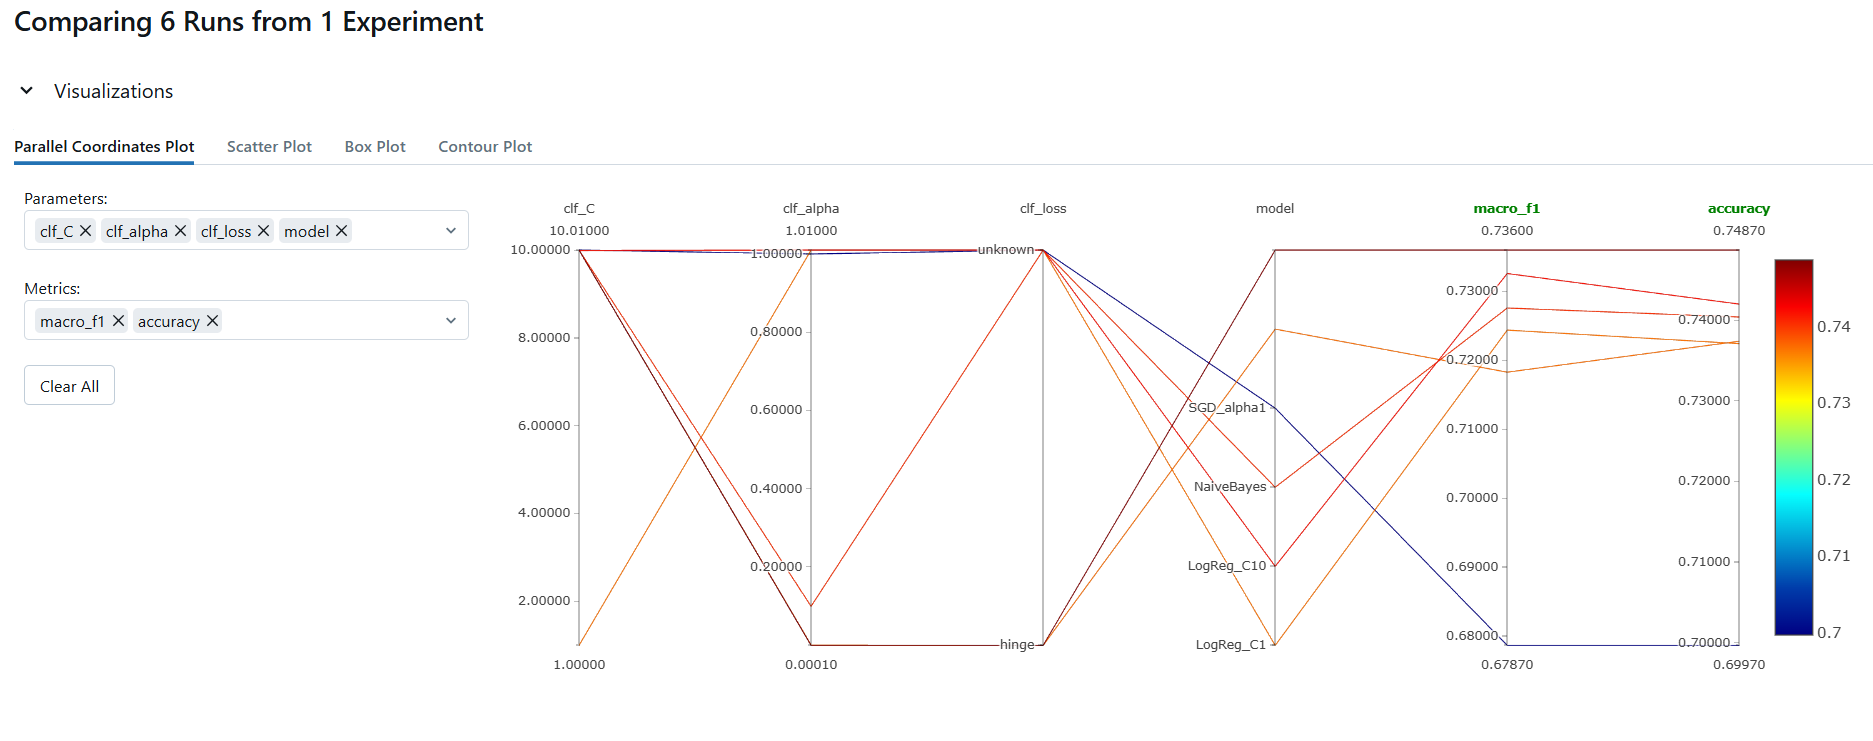
\includegraphics[width=\linewidth, height=0.36\textheight, keepaspectratio]{compare_models.png}\\[0.2cm]
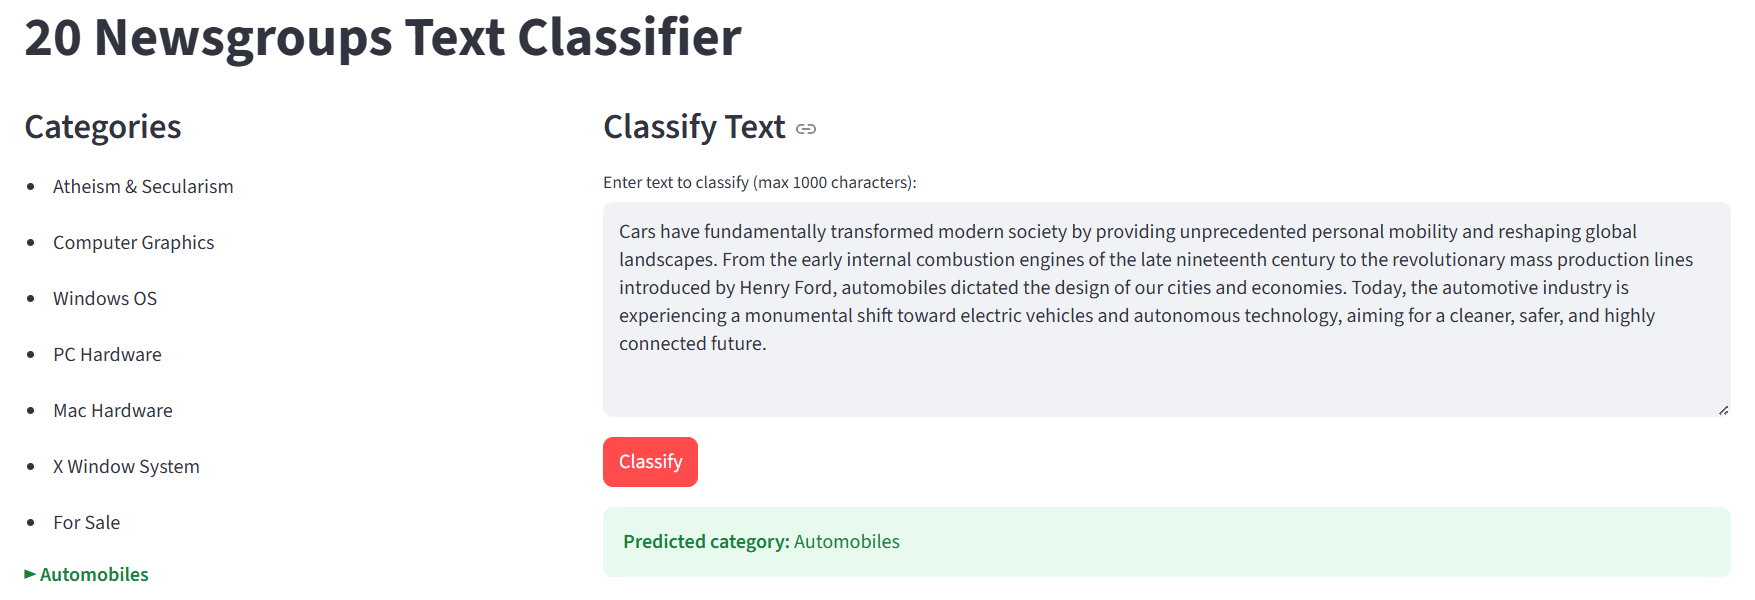
\includegraphics[width=\linewidth, height=0.36\textheight, keepaspectratio]{streamlit.png}
\end{column}
\end{columns}
\end{frame}

% ================================================================
%  SLIDE 6 — Takeaways
% ================================================================
\begin{frame}{Bilan \& Perspectives}
\small
\begin{columns}[T]
\begin{column}{0.48\textwidth}
\textbf{\faCheckCircle[regular]\; Ce que nous avons construit}
\begin{enumerate}\setlength{\itemsep}{1pt}
  \item Pipeline automatis\'e~: t\'el\'echargement, pr\'etraitement, entra\^inement
  \item 6 mod\`eles compar\'es par ex\'ecution dans MLflow
  \item Promotion du champion emp\^echant les r\'egressions
  \item API REST + interface web pour les pr\'edictions
  \item D\'eploiement Docker Compose \textbf{ou} K8s (Kind)
\end{enumerate}
\end{column}

\begin{column}{0.48\textwidth}
\textbf{\faRocket\; Perspectives}
\begin{itemize}\setlength{\itemsep}{1pt}
  \item Mod\`eles deep learning (BERT)
  \item D\'etection de d\'erive des donn\'ees
  \item CI/CD via GitHub Actions
  \item PostgreSQL pour Airflow \`a l'\'echelle
  \item Tests A/B entre champions
\end{itemize}
\end{column}
\end{columns}

\vspace{0.4em}
\centering
{\Large \alert{Merci --- Questions~?}}
\end{frame}

\end{document}